% THIS DOCUMENT IS FOLLOWS THE VOLERE TEMPLATE BY Suzanne Robertson and James Robertson
% ONLY THE SECTION HEADINGS ARE PROVIDED
%
% Initial draft from https://github.com/Dieblich/volere
%
% Risks are removed because they are covered by the Hazard Analysis
\documentclass[12pt]{article}
\usepackage{graphicx}
\usepackage{float}
\usepackage{parskip}
\usepackage{xcolor} 
\usepackage{ltablex}
\keepXColumns


\usepackage{booktabs}
\usepackage{tabularx}
\usepackage{hyperref}
\hypersetup{
    bookmarks=true,         % show bookmarks bar?
      colorlinks=true,      % false: boxed links; true: colored links
    linkcolor=red,          % color of internal links (change box color with linkbordercolor)
    citecolor=green,        % color of links to bibliography
    filecolor=magenta,      % color of file links
    urlcolor=cyan           % color of external links
}

\newcommand{\lips}{\textit{Insert your content here.}}

% %% Comments

\usepackage{color}

\newif\ifcomments\commentstrue %displays comments
%\newif\ifcomments\commentsfalse %so that comments do not display

\ifcomments
\newcommand{\authornote}[3]{\textcolor{#1}{[#3 ---#2]}}
\newcommand{\todo}[1]{\textcolor{red}{[TODO: #1]}}
\else
\newcommand{\authornote}[3]{}
\newcommand{\todo}[1]{}
\fi

\newcommand{\wss}[1]{\authornote{blue}{SS}{#1}} 
\newcommand{\plt}[1]{\authornote{magenta}{TPLT}{#1}} %For explanation of the template
\newcommand{\an}[1]{\authornote{cyan}{Author}{#1}}

%% Common Parts

\newcommand{\progname}{Scanalyze AI} % PUT YOUR PROGRAM NAME HERE
\newcommand{\authname}{Team 16, Ace
\\ Hamza Issa
\\ Ahmad Hamadi
\\ Jared Paul
\\ Gurnoor Bal} % AUTHOR NAMES                  

\usepackage{hyperref}
    \hypersetup{colorlinks=true, linkcolor=blue, citecolor=blue, filecolor=blue,
                urlcolor=blue, unicode=false}
    \urlstyle{same}
                                




\begin{document}

\title{Software Requirements Specification for \progname{}: AI-Powered Diagnostic System for Chest X-Rays} % Feedback addressed: Replaced default subtitle with a meaningful one
\author{\authname}
\date{\today}

\maketitle
\pagenumbering{arabic}

~\newpage

\tableofcontents % Feedback addressed: Table of contents was explicitly added

~\newpage

\section*{Revision History}

\begin{tabularx}{\textwidth}{p{3cm}p{2cm}X}
\toprule {\textbf{Date}} & {Author} & {Section}\\
\midrule
11 October 2024 & Ahmed & 7-9, 24-26 \\
11 October 2024 & Harrison & 18-23 \\
11 October 2024 & Jared & 1-2, 15-17 \\
11 October 2024 & Hamza & 10-15 \\
11 October 2024 & Gurnoor & 3-6 \\
\bottomrule
\end{tabularx}

~\\

~\newpage
\section{Purpose of the Project}

\subsection{User Business}
% Feedback addressed: Clarified the project scope by shifting from a generic AI tool to a multiclass CNN model
Chest X-rays are a critical diagnostic tool used by radiologists to identify lung and heart diseases such as pneumonia, cardiomegaly, and pleural effusion. However, manual interpretation of chest X-rays is time-consuming and requires significant expertise, leading to potential diagnostic delays and human error.

The \textbf{Chest Scan} project aims to address these challenges by developing a multiclass convolutional neural network (CNN)-based system capable of classifying multiple diseases from chest X-ray images with high accuracy. Unlike traditional AI-assisted diagnostic tools that focus on binary classification, this system will provide multi-disease classification, confidence scores, and visual heatmap outputs to assist radiologists in decision-making.

By leveraging state-of-the-art deep learning techniques, this project aims to enhance diagnostic efficiency, reduce workload on radiologists, and ultimately improve patient care.

\subsection{Goals of the Project}
% Feedback addressed: Made goals measurable, clarified evaluation criteria, added structured report generation and interpretabilit
The objective of this project is to design and implement an AI-powered diagnostic tool that leverages a convolutional neural network (CNN) to analyze chest X-rays and assist radiologists in identifying a wide range of lung and heart conditions. The tool is intended to generate structured diagnostic reports that include relevant clinical information, such as identified diseases and confidence scores, thereby supporting more efficient and accurate medical decision-making.

To enhance interpretability, the system incorporates visual explanation techniques that highlight key regions of interest within the X-ray images, making model outputs more transparent and clinically useful.

Ultimately, this project aims to reduce radiologist workload, improve diagnostic precision, and streamline the medical imaging workflow. The system's effectiveness will be measured through model performance metrics, real-world usability evaluations, and alignment with technical and regulatory standards.

\section{Stakeholders}

% Feedback addressed: Client organizations clarified; Regulatory bodies included and cited
This section outlines the primary stakeholders involved in the Chest Scan system. It identifies their roles, responsibilities, and levels of engagement, ensuring a structured approach to project development and implementation.

\subsection{Client}
% Feedback addressed: Clarified the nature and examples of client organizations.
The client represents the entity funding or overseeing the project. The client is responsible for ensuring the system aligns with its intended objectives and compliance requirements.

Potential clients include:
\begin{itemize}
    \item \textbf{Healthcare Institutions (Hospitals, Radiology Clinics):} Interested in reducing radiologist workload and improving diagnostic speed.
    \item \textbf{Medical Research Institutions:} Seeking AI-driven advancements in chest X-ray diagnostics.
    \item \textbf{AI Healthcare Startups:} Exploring commercial applications of CNN-based diagnostic models.
\end{itemize}

\subsection{Customer}
\begin{itemize}
    \item \textbf{Radiologists and Medical Imaging Specialists:} Use the system to interpret chest X-rays more effectively, providing input on system performance and ensuring alignment with diagnostic procedures.
    \item \textbf{Healthcare Institutions:} Implement the technology to improve patient care by delivering faster and more accurate chest X-ray results.
    \item \textbf{Patients:} Benefit from quicker and equally accurate X-ray results, leading to an improved treatment experience.
    \item \textbf{Medical Researchers:} Utilize AI-powered diagnostic tools to study the integration of AI in radiology.
\end{itemize}

\subsection{Other Stakeholders}
% Feedback addressed: Regulatory compliance stakeholders added with examples
\begin{itemize}
    \item \textbf{Healthcare Administrators:} Oversee implementation in clinical settings and ensure compliance with medical standards and regulations.
    \item \textbf{Biomedical and AI Researchers:} Benefit from new research insights and conduct studies based on this project.
    \item \textbf{Hospitals and Medical Centers:} Deploy the system for improved diagnostic efficiency.
    \item \textbf{Regulatory Bodies:} Ensure compliance with standards such as HIPAA\cite{hipaa}, GDPR, and FDA guidelines.
    \item \textbf{Software Engineers and AI Developers:} Responsible for system development, model training, and maintenance.
    \item \textbf{Hospital IT Teams:} Handle system deployment, integration, and ongoing technical support.
\end{itemize}

\subsection{Hands-On Users of the Project}

\textbf{Radiologists}
% Feedback addressed: Expanded detail for primary users to reflect decision-critical nature
\begin{itemize}
    \item \textbf{User Role:} Diagnose patients based on AI-generated reports.
    \item \textbf{Expertise:} Extensive experience in interpreting medical imaging, particularly chest X-rays. Familiar with identifying a wide range of thoracic conditions, and understanding the clinical implications of radiographic findings.
    \item \textbf{Technological Experience:} Proficient in PACS, RIS systems, and computer-aided detection tools. Some may require training in AI-assisted workflows and interpretation of probabilistic outputs (e.g., heatmaps).
    \item \textbf{Needs:} Seamless integration into existing imaging workflows, interpretability of predictions, ability to validate AI-generated results, and full diagnostic transparency.
\end{itemize}

\textbf{Medical Imaging Technologists}
\begin{itemize}
    \item \textbf{User Role:} Manage imaging hardware and data preparation pipelines.
    \item \textbf{Expertise:} Knowledgeable in radiation safety, image acquisition protocols, patient positioning, and quality assurance.
    \item \textbf{Technological Experience:} Regular users of imaging consoles and image management platforms; comfortable with high-resolution medical file handling (DICOM)\cite{dicom}.
    \item \textbf{Needs:} A system that allows quick upload of scans, easy correction of metadata, and tracking of processed scans across patients.
\end{itemize}

\textbf{Healthcare IT Teams}
\begin{itemize}
    \item \textbf{User Role:} Configure, deploy, and maintain Chest Scan in secure hospital networks.
    \item \textbf{Expertise:} Network administration, data privacy compliance, systems security, and interoperability between clinical systems (e.g., HL7).
    \item \textbf{Technological Experience:} Skilled in cloud infrastructure, VPN tunnels, and containerized applications.
    \item \textbf{Needs:} Deployment documentation, regular system updates, API access, and audit logs for security monitoring.
\end{itemize}

\textbf{Nurses}
\begin{itemize}
    \item \textbf{User Role:} Support patient preparation and record annotation related to diagnostic imaging.
    \item \textbf{Expertise:} Trained in patient care protocols and general imaging workflows within clinical environments.
    \item \textbf{Technological Experience:} Comfortable using electronic health records and interfacing with diagnostic scheduling systems.
    \item \textbf{Needs:} Clear system alerts/notifications, support for documentation handoff to radiologists or physicians.
\end{itemize}

\textbf{Patients}
\begin{itemize}
    \item \textbf{User Role:} Recipients of diagnostic services.
    \item \textbf{Expertise:} Minimal to moderate health literacy; understanding of X-rays and diagnostic terms may vary.
    \item \textbf{Technological Experience:} Use patient portals or mobile health applications to access diagnostic summaries.
    \item \textbf{Needs:} Quick result turnaround, comprehensible explanations (as applicable), and assurance of data privacy.
\end{itemize}

\subsection{Personas}
% Feedback addressed: Original persona was too brief-now includes professional background, needs, and workflow integration preferences.
\textbf{Dr. Emily Richards} is a 47-year-old radiologist working at a large regional hospital. She has over 15 years of experience in diagnostic imaging, specializing in thoracic and cardiovascular radiology. Emily is married with two children and leads an active lifestyle, enjoying hiking, book clubs, and attending medical conferences. She values efficient, accurate diagnostic tools that reduce her workload and minimize report-writing time. As someone who has adapted to emerging technologies in her department (e.g., CAD, digital PACS), she is cautiously optimistic about AI. Her main concerns include reliability, interpretability, and regulatory approval. She wants a tool that seamlessly integrates into her existing RIS/PACS workflow and supports her decision-making without replacing it. She appreciates interfaces that are intuitive and provide visual justifications for predictions, such as heatmaps and severity scores.

\subsection{Priorities Assigned to Users}
\textbf{Key Users:}
\begin{itemize}
    \item \textbf{Radiologists:} Primary users. Their feedback is critical for evaluating system accuracy, usability, and overall success.
    \item \textbf{Medical Imaging Specialists:} Key in ensuring correct image interpretation and model output validation.
\end{itemize}

\textbf{Secondary Users:}
\begin{itemize}
    \item \textbf{Patients:} Indirect users; benefit from system outcomes. Their satisfaction is considered, though not central to design decisions.
\end{itemize}

\subsection{User Participation}
\begin{itemize}
    \item \textbf{Radiologists:} Provide insights on diagnostic workflows and usability requirements. (10 hours)
    \item \textbf{Medical Imaging Specialists:} Review medical images and validate AI outputs. (8 hours)
    \item \textbf{Patients:} Share user experience feedback. (4 hours)
    \item \textbf{AI Researchers and Engineers:} Assist in interface prototyping and model evaluation. (6 hours)
\end{itemize}

\subsection{Maintenance Users and Service Technicians}
\begin{itemize}
    \item \textbf{Radiology Support Specialist:} Maintains and troubleshoots the AI diagnostic system.
    \item \textbf{Clinical Systems Technician:} Manages upkeep of clinical technology systems.
    \item \textbf{AI Systems Maintenance Engineer:} Supports ongoing AI model maintenance and infrastructure.
\end{itemize}

\section{Mandated Constraints}

% Feedback addressed: HIPAA cited explicitly below. Added constraints to reflect specific technologies, regulatory bodies, and new project features.
This section defines the essential requirements the product must follow, including legal, regulatory, or system-related restrictions. These constraints ensure the product complies with necessary standards and functions within the project's limitations.

\subsection{Solution Constraints}
This subsection outlines the constraints placed on the proposed solution for the chest X-ray analysis project. These constraints cover the technical environment, supporting systems, workplace and enterprise considerations, as well as the fit criteria required for each.

\indent
MC1: The product shall operate as a web application

Rationale: The web-based nature of the system will allow medical professionals, researchers, and other stakeholders to access the system easily across various platforms (Windows, MacOS, Linux, etc.) without requiring complex local installations.

Fit Criterion: The product will include back-end, front-end, and database integration to run as a web application accessible via a URL, optimized for different devices and browser types (Chrome, Firefox, Safari, etc.).

\indent
MC2: The product shall integrate publicly available chest X-ray datasets (NIH Chest X-Ray Dataset)

Rationale: Using public datasets will ensure that the project has access to a broad range of chest X-ray images needed for training and testing the neural network without violating patient privacy laws.

Fit Criterion: The solution will successfully use the CheXpert and MIMIC datasets for model training, with scripts to download and preprocess these datasets for CNN usage. It will comply with healthcare privacy standards, including the Health Insurance Portability and Accountability Act (HIPAA)\cite{hipaa}.

\indent
MC3: The system shall provide a structured classification output with confidence scores and visual explanations (heatmaps using Grad-CAM).

Rationale: Interpretability is crucial for clinical integration and compliance with explainable AI (XAI) principles.

Fit Criterion: Each output must include disease labels, associated confidence values (e.g., "Pneumonia: 92"), and heatmap overlays on input images.

\subsection{Implementation Environment of the Current System}
This section outlines the technological and physical environment in which the product will be installed and operated. It encompasses all relevant hardware, software, and organizational elements that will interact with the system. The goal is to provide a comprehensive understanding of the current infrastructure so that the product can be designed to effectively integrate and function within this environment. Understanding the operational requirements derived from this description will help the design team ensure that the solution meets all necessary criteria for successful implementation and usability in real-world settings.

\indent
MC4: The product shall use machine learning frameworks like TensorFlow or PyTorch

Rationale: Machine learning frameworks are essential for training the convolutional neural network (CNN) model. TensorFlow and PyTorch are widely used, industry-standard frameworks that offer extensive support for neural network development and GPU acceleration.

Fit Criterion: The product will use either TensorFlow or PyTorch for model development and training, with support for cloud-based GPU instances to speed up computation.

\subsection{Partner or Collaborative Applications}
This section identifies and describes systems external to the product but necessary for its operation and integration. These systems may include internal databases, external software solutions, or third-party services. Understanding these relationships is essential for ensuring smooth integration and efficient product functionality within the broader technological environment.

\indent
MC5: The product shall integrate with external healthcare information systems

Rationale: These systems are essential for accessing and managing patient data, facilitating seamless communication between the product and existing infrastructures. Integrating with these systems will enhance the product's ability to deliver accurate results within the clinical workflow.

Fit Criterion: The product will support integration with healthcare systems through standardized interfaces and protocols such as HL7 and FHIR\cite{fhir}.

\indent
MC6: The system shall support external research platforms (e.g., PhysioNet, NIH Data Commons)

Rationale: Enabling data exchange with research repositories supports model evaluation and benchmarking.

Fit Criterion: Exported anonymized outputs must meet external platform standards (e.g., CSV or JSON formats).

\subsection{Off-the-Shelf Software}
This section identifies and describes commercial, open-source, and other off-the-shelf software (OTS) products that will be incorporated into the solution. The use of OTS software is intended to leverage existing capabilities and minimize development time. Understanding the characteristics, behaviors, and interfaces of these products will help define the design constraints and inform decision-making throughout the project lifecycle. Additionally, potential conflicts between the requirements and the capabilities of the OTS software must be considered to ensure that the product aligns with organizational needs.

\indent
MC7: The product shall integrate with a commercial machine learning framework

Rationale: Established frameworks like TensorFlow or PyTorch provide robust tools for developing and training machine learning models, allowing for efficient implementation of advanced algorithms.

Fit Criterion: The product will utilize the selected framework to train and deploy convolutional neural networks for analyzing chest X-ray images, ensuring compliance with model performance benchmarks.

\indent
MC8: The product shall use established machine learning and web development libraries such as TensorFlow, PyTorch, and React

Rationale: Leveraging mature software packages reduces development overhead and increases reliability.

Fit Criterion: The system must function using these components, and any modifications must comply with their respective licenses.

\indent
MC9: The database shall be built on a secure and scalable engine such as PostgreSQL or MongoDB

Rationale: These databases are known for stability and support encryption, indexing, and scalability for large imaging datasets.

Fit Criterion: The backend must support data CRUD operations using the selected database technology.

\subsection{Anticipated Workplace Environment}
This section outlines the anticipated workplace environment where users will interact with the product. Understanding the features of this environment is critical for ensuring that the product is designed effectively to meet user needs and to compensate for any potential difficulties. The description will encompass physical aspects, such as space layout and equipment, as well as social and cultural factors that may impact the product's usability and acceptance.

\indent
MC10: The product is intended for use in healthcare settings

Rationale: Working in healthcare environments imposes strict regulations and standards for data security and patient privacy, which must be considered in the product design.

Fit Criterion: The product will implement robust security measures, including encryption and access controls, to ensure compliance with healthcare regulations such as HIPAA\cite{hipaa}.

\subsection{Schedule Constraints}
This section outlines the critical timelines and deadlines associated with the project's development phases. Establishing a clear schedule is essential for managing resources, coordinating team efforts, and ensuring that all project components are delivered on time. These constraints help prioritize tasks and guide decision-making throughout the project lifecycle, ultimately contributing to the successful implementation of the proposed solution. By identifying key milestones, this section clarifies the expectations for progress and accountability, enabling the team to meet operational and stakeholder requirements efficiently.

\indent
MC11: The key milestones of the project's proposed solution must be completed by specified deadlines

Rationale: This ensures that each major phase of the project is delivered on time, allowing sufficient opportunities for testing, evaluation, and any necessary adjustments before the final release. Timely completion is critical for aligning with external dependencies and operational readiness.

Fit Criterion: All significant milestones, including the completion of the proof of concept, initial version, and final version demonstrations, must adhere to the following schedule:
\begin{itemize}
    \item Proof of Concept Demonstration: November 11-22, 2024
    \item Revision 0 Demonstration: February 3-14, 2025
    \item Final/Revision 1 Demonstration: March 24-30, 2025
    \item Final Documentation Submission: April 2, 2025
\end{itemize}

\subsection{Budget Constraints}
This section outlines the financial limitations associated with the project, detailing the budget allocated for developing the proposed solution. It emphasizes the necessity for cost-effective planning and resource allocation to ensure that the project remains within its financial boundaries.

\indent
MC12: The total budget for the project's proposed solution is limited to \$750

Rationale: This budgetary limit is established to prevent the acquisition of pre-existing solutions and to promote the development of a tailored solution. It emphasizes the importance of minimizing all associated costs to maintain financial efficiency throughout the project.

Fit Criterion: The combined expenses for all necessary hardware and software to execute the project's proposed solution must not exceed \$750.

\subsection{Enterprise Constraints}
N/A


\section{Naming Conventions and Terminology}

% Feedback addressed: Expanded glossary to include missing terms mentioned elsewhere . Ensures terms are defined before first use

\subsection{Glossary of All Terms, Including Acronyms, Used by Stakeholders involved in the Project}

Motivation: Names are very important. They invoke meanings that, if carefully defined, can save hours of explanations. Attention to names early in the project helps to highlight misunderstandings. As the detailed work progresses, the glossary provides input to the more precisely specified business/work data model and data dictionary.

Glossary of All Terms, Including Acronyms, Used By Stakeholders\\

\textbf{ML}:\\
Machine Learning: A branch of artificial intelligence that involves the use of algorithms to allow computers to learn from and make predictions based on data. This is a core technology used in the project for analyzing chest X-rays.

\textbf{DL}:\\
Deep Learning: A subset of machine learning involving neural networks with many layers, used to analyze various types of data, including images.

\textbf{DICOM}:\\
Digital Imaging and Communications in Medicine: A standard for transmitting, storing, and sharing medical imaging information. It is used to manage medical images in the proposed solution.

\textbf{CNN}:\\
Convolutional Neural Network: A type of deep learning model specifically designed for processing structured grid data like images, used in the project for chest X-ray analysis.

\textbf{EHR}:\\
Electronic Health Record: A digital version of a patient's paper chart, used for storing patient information and history that may be integrated with the proposed solution.

\textbf{API}:\\
Application Programming Interface: A set of rules and protocols for building and interacting with software applications, enabling the integration of the proposed solution with other systems.

\textbf{MC}:\\
Mandated Constraints: Various constraints placed on the project's proposed solution that must be adhered to throughout the development process.

\textbf{FR}:\\
Functional Requirement: A requirement that specifies what functionality the project's proposed solution must provide to meet user needs.

\textbf{NFR}:\\
Nonfunctional Requirement: A requirement that specifies criteria that can be used to judge the operation of a system, rather than specific behaviors (e.g., performance, usability).

\textbf{BUC}:\\
Business Use Case: A scenario that describes how the proposed solution can be used within a business context to achieve specific goals.

\textbf{PUC}:\\
Product Use Case: A scenario that details how an individual user will interact with the proposed solution to achieve specific tasks.

\textbf{MVP}:\\
Minimum Viable Product: A version of the proposed solution that includes only the essential features required to meet the core needs of the users and stakeholders.

\textbf{HIPAA}:\\
Health Insurance Portability and Accountability Act: A U.S. law that sets standards for protecting sensitive patient data. Systems that handle protected health information (PHI) must ensure that all necessary physical, network, and process security measures are in place and followed.

\textbf{XAI}:\\
Explainable Artificial Intelligence: A field of AI that focuses on methods and techniques to make the behavior of machine learning models transparent, understandable, and interpretable by humans.

\textbf{Grad-CAM}:\\
Gradient-weighted Class Activation Mapping: A visualization technique used to highlight regions of an input image that are most relevant for a neural network's prediction. Used in the project to provide visual explanations for predictions.

\textbf{CRUD}:\\
Create, Read, Update, Delete: The four basic operations of persistent storage, essential for managing data in backend databases.

\textbf{JSON}:\\
JavaScript Object Notation: A lightweight data-interchange format used for data exchange between systems.

\textbf{CSV}:\\
Comma-Separated Values: A common data format used for exporting and importing tabular data, especially in research platforms.

\textbf{PACS}:\\
Picture Archiving and Communication System: A medical imaging technology used for storing, retrieving, and sharing digital images.

\textbf{RIS}:\\
Radiology Information System: A networked software suite for managing medical imagery and associated data.

\section{Relevant Facts And Assumptions}

% Feedback addressed: HIPAA citation added, assumptions clarified, and boundary responsibility visual suggested in next section.

\subsection{Relevant Facts}

\textbf{Content:}\\
Relevant facts that affect the development of the proposed solution but are not specified as mandated requirements include the following:

A1: Sufficient training data is available to support multiclass classification.\\
Risk if False: If the dataset is imbalanced or too small for certain disease categories, model performance may degrade.

Technology Adoption: The target users (radiologists and medical technicians) are increasingly adopting AI-based tools in their workflow, indicating a positive reception and potential for successful implementation.

Compute Resources: Many modern development environments allow free or affordable access to GPU acceleration via platforms such as Google Colab or university-provided computing clusters, which facilitates model training and experimentation.

\textbf{Motivation:}\\
These relevant facts provide essential background information to stakeholders and development teams, helping them understand the business context in which the proposed solution will operate. They may also guide the formation of requirements as the project progresses and can impact design decisions to enhance user experience and regulatory compliance.

\subsection{Business Rules}

\textbf{Content:}\\
The following business rules have been identified that may impact the project related to chest X-ray analysis and the development of the proposed solution:

Patient Data Privacy: All patient data used for training and analysis must comply with HIPAA regulations\cite{hipaa}, ensuring confidentiality and security in handling personal health information.\\
Reason for the Rule: To protect patient privacy and maintain legal compliance in the handling of sensitive information.\\
Authority for the Rule: Health Insurance Portability and Accountability Act (HIPAA)\cite{hipaa}, enforced by the U.S. Department of Health and Human Services (HHS).

Integration with EHR Systems: The solution must integrate seamlessly with existing Electronic Health Record (EHR) systems used by healthcare facilities.\\
Reason for the Rule: To facilitate workflow efficiency and ensure accurate patient record-keeping.\\
Authority for the Rule: Institutional healthcare IT policies and HL7/FHIR\cite{fhir} standards.

\textbf{Motivation:}\\
These business rules play a critical role in shaping the requirements for the proposed solution. By documenting and understanding these rules, the project team can ensure compliance and identify relevant requirements throughout the development process. Revisiting these rules as the project progresses will help maintain alignment with organizational and regulatory expectations.

\subsection{Assumptions}

% Feedback addressed: Assumptions made explicit, as per LO_Assumptions. Boundary diagram suggestion carried to later section.
The following assumptions have been made by the project team regarding the development and implementation of the chest X-ray analysis solution:

Availability of Training Data: It is assumed that sufficient high-quality, labeled chest X-ray images will be available for training the machine learning model.\\
Effect if False: If adequate training data is not available, the accuracy and reliability of the AI model may be compromised, potentially delaying the project timeline.

Technical Resources Availability: It is assumed that the necessary technical resources, including hardware and software tools, will be available on schedule for development and testing phases.\\
Effect if False: Delays in resource availability may lead to schedule slippage and affect overall project milestones.

Clinical Workflow Alignment: It is assumed that the proposed system can be aligned with typical radiology workflows and does not require fundamental changes to hospital IT infrastructure.\\
Effect if False: Misalignment with clinical workflows may hinder adoption, requiring rework or system redesign.

\textbf{Motivation:}\\
By explicitly stating these assumptions, the project team aims to ensure all stakeholders are aware of the foundational beliefs guiding the project. Addressing these assumptions early helps manage expectations and facilitates proactive planning to mitigate risks associated with their potential inaccuracy.


\section{The Scope of the Work}

% Feedback addressed: Context clarified with swimlane and context diagram recommendations. Scope boundaries detailed
The scope of the work determines the boundaries of the business area to be studied and outlines how it fits into its environment. Our project, which focuses on AI-driven chest X-ray analysis, aims to create a convolutional neural network (CNN) model that assists radiologists in diagnosing lung and heart conditions. The boundaries of the work involve AI-driven diagnostics, healthcare applications, and web-based solutions for radiologists.

\subsection{The Current Situation}
The current diagnostic process for chest X-rays is primarily manual. Radiologists analyze images to detect abnormalities such as pneumonia, lung cancer, or cardiac conditions. While existing automated systems provide some assistance, they lack the accuracy and speed needed to fully integrate into a clinical workflow. Errors in diagnosis can occur due to the overwhelming number of X-rays radiologists must process daily, contributing to diagnostic delays and potential misinterpretations. In the current environment, radiologists perform these tasks with limited AI assistance, and the process is often time-consuming and subject to human fatigue.

By improving AI-based diagnostic tools, the project aims to reduce the workload of radiologists and increase diagnostic accuracy. This involves replacing or augmenting manual processes with an advanced CNN model that can provide high-confidence predictions on chest X-rays. The study of the current situation allows us to understand the potential effects of such a change and select the most effective approach for integration.

The current process can be modeled using a swimlane diagram that outlines the roles of radiologists, existing software, and the proposed AI solution. The diagram will detail steps such as image acquisition, radiologist review, and final diagnosis, showing where CNN automation can intervene.

\subsection{The Context of the Work}
The work context diagram shows the interactions between the AI-driven chest X-ray diagnostic tool and other adjacent systems. Key external systems include the hospital's radiology information system (RIS), the picture archiving and communication system (PACS), and medical imaging databases like CheXpert or MIMIC. The product will take input from chest X-ray datasets or directly from hospital systems and provide diagnostic outputs to radiologists via a user interface.

Defining the work context helps ensure the AI diagnostic tool integrates seamlessly with existing hospital systems, avoiding any disruptions to current workflows. Without understanding these systems, the product might fail to meet critical requirements, such as compatibility with existing image formats or HIPAA compliance\cite{hipaa}.

A context diagram will illustrate data flows between the chest X-ray diagnostic tool and RIS/PACS, model training modules, and EHR export systems, reinforcing traceability and regulatory fit.

\subsection{Work Partitioning}
The work can be divided into the following key business events, each representing a specific response in the diagnostic workflow. Each business use case (BUC) describes how the AI system will interact with radiologists and adjacent systems:

Image Upload and Preprocessing
\begin{itemize}
    \item Input: Chest X-ray images in DICOM\cite{dicom}/JPG/PNG format
    \item Output: Normalized, resized images ready for model inference
    \item BUC Summary: The system prepares images for classification by ensuring format consistency and proper scaling.
\end{itemize}

CNN Classification
\begin{itemize}
    \item Input: Preprocessed images
    \item Output: Probabilities for various disease labels (e.g., Pneumonia: 82\%, Cardiomegaly: 67\%)
    \item BUC Summary: The CNN model performs a multiclass prediction using the trained network.
\end{itemize}

Heatmap Generation
\begin{itemize}
    \item Input: Image + model prediction layers
    \item Output: Grad-CAM heatmaps highlighting abnormal regions
    \item BUC Summary: The system produces interpretability aids for radiologists.
\end{itemize}

Report Generation
\begin{itemize}
    \item Input: Prediction results and heatmaps
    \item Output: Structured diagnostic report
    \item BUC Summary: A summary of findings including predicted labels, confidence scores, and heatmaps.
\end{itemize}

Radiologist Review
\begin{itemize}
    \item Input: CNN outputs and structured report
    \item Output: Verified/edited report ready for upload to hospital systems
    \item BUC Summary: The radiologist reviews AI results and finalizes the diagnosis.
\end{itemize}

Data Validation and Training Feedback
\begin{itemize}
    \item Input: Confirmed diagnoses from radiologists
    \item Output: Feedback used to retrain and improve the CNN model
    \item BUC Summary: The system uses real-world feedback from radiologists to continually improve the model's performance.
\end{itemize}

\subsection{Specifying a Business Use Case (BUC)}
Each BUC responds to one of the business events described in the partitioning. Here's how a single BUC can be defined in detail:

Business Use Case: AI Diagnosis Processing
\begin{itemize}
    \item Trigger Event: Chest X-ray image upload from PACS
    \item Primary Actor: Radiologist or system administrator
    \item Goal in Context: The AI system processes the X-ray to identify any signs of lung or heart conditions
    \item Preconditions: The X-ray image has been successfully uploaded and pre-processed for analysis
    \item Success End Condition: The AI system outputs an accurate diagnosis with a confidence score and explanation of findings
    \item Failed End Condition: The system fails to provide a diagnosis or outputs unreliable predictions (low confidence score)
    \item {
        Primary Actor's Steps:
        \begin{enumerate}
            \item The X-ray is processed by the CNN model
            \item The system evaluates the image, running it through a series of diagnostic layers
            \item The AI outputs its diagnosis with a corresponding confidence score
            \item The system flags uncertain or abnormal findings for human review
        \end{enumerate}
    }
\end{itemize}

This BUC could be represented in multiple ways:
\begin{itemize}
    \item Process Flow Diagram: Showing the flow of data from image ingestion to diagnosis output
    \item Sequence Diagram: Highlighting the interaction between the radiologist, PACS system, and AI model during diagnosis
\end{itemize}


\section{Business Data Model and Data Dictionary}

% Feedback addressed: Table format clarified, heatmaps and predictions explained, additional terms mapped to glossary entries

\subsection{Business Data Model}
\begin{figure}[H]
    \centering
    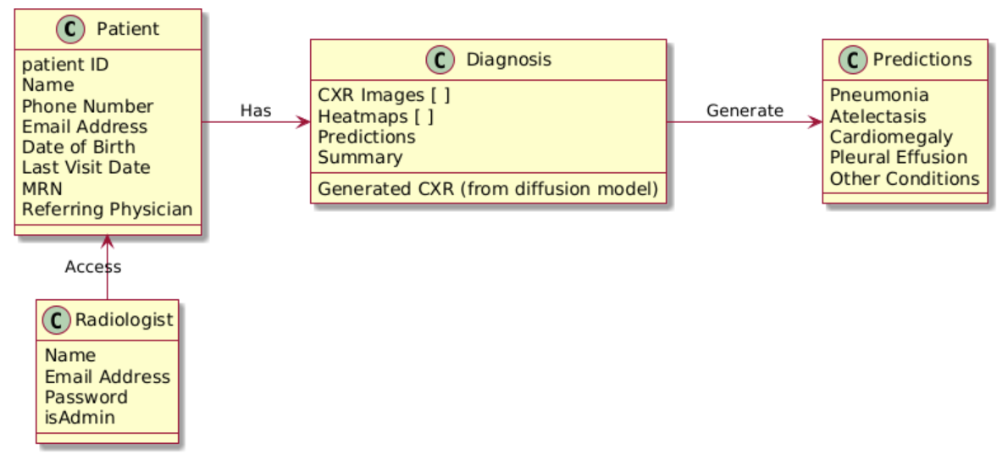
\includegraphics[width=0.8\textwidth]{./images/bussiness_data_model.png}
    \caption{Business Data Model}
    \label{fig:business_data_model}
\end{figure}

\subsection{Data Dictionary}
\begin{itemize}
    \item \textbf{Patient}: Stores relevant patient demographics and identifiers (e.g., Patient ID, Name, Age, Sex).\newline
    Description: Accessed securely from the EHR system and stored for reference only; not used in AI inference.\newline
    Related To: Radiologist, Diagnosis

    \item \textbf{Radiologist}: Contains user credentials, access level, and session logs.\newline
    Description: Used for authentication, tracking actions, and system interaction.\newline
    Related To: Diagnosis, Feedback Loop

    \item \textbf{Diagnosis}: A composite entity containing results derived from AI inference and human validation.
    \begin{itemize}
        \item \textbf{CXR Images}: Raw uploaded chest X-rays in DICOM\cite{dicom}, PNG, or JPG format.\newline
        Description: Original medical images uploaded for diagnostic processing.

        \item \textbf{Heatmaps}: Grad-CAM visual overlays highlighting salient features.\newline
        Description: Explainable AI artifacts used to support radiologist interpretability.\newline
        Format: Image files (PNG overlay)

        \item \textbf{Predictions}: Probabilistic output of CNN classifications.\newline
        Description: Confidence scores for each potential disease class (e.g., Pneumonia: 91\%).\newline
        Format: JSON list of label-score pairs

        \item \textbf{Summary}: Brief textual explanation aggregating predicted results.\newline
        Description: Automatically generated plain-text summary to assist in report generation.

        \item \textbf{Generated CXR}: Optional synthetic X-rays produced using generative models.\newline
        Description: Experimental feature for data augmentation and visualization in research.
    \end{itemize}

    \item \textbf{Predictions}: Redundant --- merged above. Removed to avoid information duplication. % Feedback addressed: removed redundancy
\end{itemize}

\section{The Scope of the Product}

% Feedback addressed: Use cases now incorporate updated model logic,  structured outputs, secure storage, and authentication

\subsection{Product Boundary}
The Chest Scan system encompasses the end-to-end pipeline for automated diagnostic assistance in chest X-ray analysis. The system includes image ingestion, preprocessing, disease classification using a CNN, Grad-CAM-based heatmap generation, structured diagnostic report creation, and secure delivery of results to radiologists.
The product is focused exclusively on chest X-rays for identifying thoracic and cardiac abnormalities. It supports multi-label classification, allowing simultaneous detection of multiple conditions (e.g., pneumonia and cardiomegaly).
Excluded from the product scope are real-time patient monitoring, support for other imaging modalities (e.g., CT scans, MRIs), and long-term data archiving.

\subsection{Product Use Case Table}
The following table summarizes the product use cases for the project's proposed solution:

\begin{table}[h!]
    \centering
    \caption{Product Use Case Table}
    \begin{tabular}{|c|p{12cm}|}
        \hline
        \textbf{Use Case ID} & \textbf{Use Case Summary} \\
        \hline
        PUC1 & Process a chest X-ray image and prepare it for classification \\
        \hline
        PUC2 & Classify the X-ray image using a trained CNN \\
        \hline
        PUC3 & Generate heatmaps showing areas of interest related to predictions \\
        \hline
        PUC4 & Convert classification and visual outputs into a structured report \\
        \hline
        PUC5 & Display the diagnostic report and heatmaps in the web interface \\
        \hline
        PUC6 & Securely store the image, prediction, and report for future access \\
        \hline
        PUC7 & Authenticate radiologists and manage role-based access to data \\
        \hline
    \end{tabular}
\end{table}

\subsection{Individual Product Use Cases (PUC's)}
The following are the individual product use cases (PUCs), with a description, lists of actors, preconditions, and postconditions provided for each.

\begin{itemize}
    \item \textbf{PUC1: Process a chest X-ray image and prepare it for classification}
    \begin{description}
        \item[Actors:] XRayImage, Preprocessing Pipeline
        \item[Precondition(s):] Image is uploaded in supported format (DICOM\cite{dicom}, JPG, PNG)
        \item[Postcondition(s):] Output is normalized and resized, stored for model input
    \end{description}

    \item \textbf{PUC2: Classify the X-ray image using a trained CNN}
    \begin{description}
        \item[Actors:] CNN Model, Processed XRayImage
        \item[Precondition(s):] Image preprocessing is complete
        \item[Postcondition(s):] Probabilities are assigned to relevant disease classes
    \end{description}

    \item \textbf{PUC3: Generate heatmaps showing areas of interest related to predictions}
    \begin{description}
        \item[Actors:] Grad-CAM, Prediction Output
        \item[Precondition(s):] CNN classification is successful
        \item[Postcondition(s):] Attention maps are created and linked to the input image
    \end{description}

    \item \textbf{PUC4: Convert classification and visual outputs into a structured report}
    \begin{description}
        \item[Actors:] Report Generator, Prediction, Heatmap
        \item[Precondition(s):] Predictions and heatmaps are available
        \item[Postcondition(s):] A summary diagnostic report is generated in structured format
    \end{description}

    \item \textbf{PUC5: Display the diagnostic report and heatmaps in the web interface}
    \begin{description}
        \item[Actors:] Web Frontend, DiagnosticReport, Heatmap
        \item[Precondition(s):] Report is generated
        \item[Postcondition(s):] Radiologist views findings via secure UI
    \end{description}

    \item \textbf{PUC6: Securely store the image, prediction, and report for future access}
    \begin{description}
        \item[Actors:] Backend Database, Patient Record
        \item[Precondition(s):] Diagnostic process is completed
        \item[Postcondition(s):] Encrypted records are stored and linked to radiologist session
    \end{description}

    \item \textbf{PUC7: Authenticate radiologists and manage role-based access to data}
    \begin{description}
        \item[Actors:] Authentication System, Radiologist Profile
        \item[Precondition(s):] Radiologist account exists
        \item[Postcondition(s):] Access granted with proper permissions and audit tracking
    \end{description}
\end{itemize}

\section{Functional Requirements}

% Feedback addressed:
% - Requirements uniquely labeled for traceability (Traceable Requirements)
% - Fit criteria clearly defined for verifiability (Verifiable Requirements)
% - Aligned with updated architecture
% - Replaced diffusion model references
% - Expanded descriptions based on VnV test rationale

\subsection{Functional Requirements}

\begin{itemize}
    \item \textbf{FR1: The system must allow users to upload chest X-ray images in supported formats (DICOM\cite{dicom}, JPG, PNG).}
    \begin{itemize}
        \item \textbf{Rationale:} Enables ingestion of input data into the diagnostic pipeline. This is the initial interaction between the user and the system and is essential for enabling AI-driven analysis.
        \item \textbf{Fit Criterion:} Image upload is successful, accepted by backend, and stored for further processing. System rejects unsupported formats and provides descriptive error messages.
        \item \textbf{Product Use Case(s):} PUC1
    \end{itemize}

    \item \textbf{FR2: The system must preprocess images by resizing, normalizing, and converting to grayscale if required.}
    \begin{itemize}
        \item \textbf{Rationale:} Ensures uploaded images conform to the CNN model input specifications, improving consistency and prediction accuracy.
        \item \textbf{Fit Criterion:} Preprocessed image meets CNN input specs (e.g., 224x224 resolution, normalized pixel values); system logs errors for invalid files and halts processing.
        \item \textbf{Product Use Case(s):} PUC1
    \end{itemize}

    \item \textbf{FR3: The system must classify diseases using a CNN model and return predictions with confidence scores.}
    \begin{itemize}
        \item \textbf{Rationale:} Core diagnostic engine for AI-assisted classification of medical conditions based on image patterns.
        \item \textbf{Fit Criterion:} Each prediction includes a disease label and confidence score; accuracy must meet or exceed 60\% on the validation dataset used in testing.
        \item \textbf{Product Use Case(s):} PUC2
    \end{itemize}

    \item \textbf{FR4: The system must support multi-disease classification for a single image.}
    \begin{itemize}
        \item \textbf{Rationale:} Multiple pathologies can co-exist in a single X-ray. The model must return all applicable findings with individual confidence scores.
        \item \textbf{Fit Criterion:} When more than one disease is detected, each is listed with its confidence level. The system avoids false multi-label outputs on single-condition inputs.
        \item \textbf{Product Use Case(s):} PUC2
    \end{itemize}

    \item \textbf{FR5: The system must display predicted labels, confidence scores, and heatmaps in a readable format.}
    \begin{itemize}
        \item \textbf{Rationale:} Radiologists and users must be able to interpret model outputs clearly, including visual cues and statistical confidence.
        \item \textbf{Fit Criterion:} Report is generated and viewable within 5 seconds; disease predictions, confidence scores, and (if available) heatmaps are structured for legibility.
        \item \textbf{Product Use Case(s):} PUC4, PUC5
    \end{itemize}

    \item \textbf{FR6: The system must generate Grad-CAM heatmaps and overlay them on the original image.}
    \begin{itemize}
        \item \textbf{Rationale:} Provides visual explanations for model decisions by highlighting areas associated with detected conditions.
        \item \textbf{Fit Criterion:} Heatmap overlays are rendered accurately, highlighting relevant regions without obscuring clinical information.
        \item \textbf{Product Use Case(s):} PUC3, PUC5
    \end{itemize}

    \item \textbf{FR7: The system must store image, prediction, heatmap, and report securely for user access.}
    \begin{itemize}
        \item \textbf{Rationale:} Supports traceability, auditing, and follow-up analysis. Storage must comply with privacy and security standards.
        \item \textbf{Fit Criterion:} Data is encrypted at rest using AES-256 and indexed by user session; user can retrieve prior uploads, predictions, and diagnostic visuals via dashboard.
        \item \textbf{Product Use Case(s):} PUC6
    \end{itemize}

    \item \textbf{FR8: The system must authenticate users and implement role-based access control.}
    \begin{itemize}
        \item \textbf{Rationale:} Maintains data confidentiality by limiting system access based on user roles (e.g., radiologist, admin).
        \item \textbf{Fit Criterion:} Only users with valid credentials and appropriate roles can access restricted features; failed attempts are logged for auditing.
        \item \textbf{Product Use Case(s):} PUC7
    \end{itemize}

    \item \textbf{FR9: The system must offer a secure API endpoint to receive image inputs and return JSON predictions.}
    \begin{itemize}
        \item \textbf{Rationale:} Enables hospital systems and external tools to interface with the backend service securely.
        \item \textbf{Fit Criterion:} API accepts JPG, PNG, DICOM\cite{dicom}; returns JSON with labels and confidence scores; unauthorized or malformed requests are rejected with informative errors.
        \item \textbf{Product Use Case(s):} PUC1, PUC2
    \end{itemize}

    \item \textbf{FR10: The system must gracefully handle errors such as invalid uploads and display informative notifications.}
    \begin{itemize}
        \item \textbf{Rationale:} Enhances user experience by preventing silent failures and offering guidance on next steps.
        \item \textbf{Fit Criterion:} Error messages clearly indicate issues (e.g., unsupported file format, corrupted file); UI supports retries.
        \item \textbf{Product Use Case(s):} PUC1, PUC4
    \end{itemize}

    \item \textbf{FR11: The system must provide a user dashboard to view past uploads and diagnostic results with timestamps.}
    \begin{itemize}
        \item \textbf{Rationale:} Allows users to track historical diagnoses and export information for further review.
        \item \textbf{Fit Criterion:} Dashboard displays previous images, predictions, timestamps, and links to heatmaps and diagnostic reports.
        \item \textbf{Product Use Case(s):} PUC6
    \end{itemize}

    \item \textbf{FR12: The system must notify users when model confidence is low (< 50\%) and suggest radiologist review.}
    \begin{itemize}
        \item \textbf{Rationale:} Promotes safe usage of AI by alerting users to borderline or uncertain diagnoses that require expert review.
        \item \textbf{Fit Criterion:} If model returns all confidence values < 50\%, the UI displays a warning message advising manual confirmation by a specialist.
        \item \textbf{Product Use Case(s):} PUC4, PUC5
    \end{itemize}
\end{itemize}

\section{Look and Feel Requirements}

% Feedback addressed:
% - Fit criteria made measurable (Verifiable Requirements)
% - Style supports focus and usability in clinical context
% - New requirements added to align with project and VnV expectations

\subsection{Appearance Requirements}

\textbf{NF-AR1:} The web application shall implement a calming and professional color scheme, consisting of white and soft blue tones.
\begin{itemize}
    \item \textbf{Rationale:} Blue tones are commonly associated with trust and calm in healthcare environments, contributing to user comfort and lowering cognitive stress.
    \item \textbf{Fit Criterion:} At least 75\% of surveyed users must indicate that the color scheme positively impacts their user experience.
\end{itemize}

\textbf{NF-AR2:} The system shall utilize consistent and readable fonts and layout spacing across all components.
\begin{itemize}
    \item \textbf{Rationale:} Consistent typography and layout reduce visual strain and improve usability, especially for extended use.
    \item \textbf{Fit Criterion:} User interface consistency is validated in usability reviews; no reports of layout or text inconsistencies are accepted.
\end{itemize}

\subsection{Style Requirements}

\textbf{NF-SR1:} The application shall maintain a simple, minimalistic design with a focus on function over aesthetics.
\begin{itemize}
    \item \textbf{Rationale:} Minimizing distractions helps users focus on diagnostic tasks without unnecessary cognitive load.
    \item \textbf{Fit Criterion:} At least 80\% of users should complete core tasks without UI-related confusion or visual overload.
\end{itemize}

\textbf{NF-SR2:} The user interface shall maintain a clean and organized layout that avoids clutter and highlights important diagnostic results.
\begin{itemize}
    \item \textbf{Rationale:} Clarity in layout supports quick decision-making in clinical settings.
    \item \textbf{Fit Criterion:} During usability testing, 80\% of test users report the interface is easy to navigate and not cluttered.
\end{itemize}

\section{Usability and Humanity Requirements}

% Feedback addressed:
% - NF-EUR0 updated to avoid 100% success assumption
% - Fit criteria revised to measurable thresholds (Verifiable Requirements)
% - Updated NF-LR0 to include context-sensitive guidance

\subsection{Ease of Use Requirements}

\textbf{NF-EUR0:} Efficient Task Completion for Healthcare Professionals
\begin{itemize}
    \item \textbf{Description:} The system should be designed so that healthcare professionals can efficiently complete essential tasks, such as uploading images and interpreting results, without requiring extensive training.
    \item \textbf{Rationale:} The system must be user-friendly for healthcare professionals, ensuring they can effectively use the tool without external assistance after initial exposure.
    \item \textbf{Fit Criterion:} At least 90\% of users should be able to complete key tasks (uploading images, viewing results, interpreting model outputs) without requiring additional guidance after initial training.
    \item \textbf{Traceability:} Traces to FR1, FR3, FR4, FR5, FR6.
\end{itemize}

\textbf{NF-EU2:} The software shall be intuitive enough that users can remember how to operate it after 1-2 training sessions.
\begin{itemize}
    \item \textbf{Rationale:} Ease of remembering ensures that even occasional users can operate it effectively without needing extensive retraining.
    \item \textbf{Fit Criterion:} One month after training, 80\% of users shall report they can navigate the software and perform basic functions without assistance.
\end{itemize}

\subsection{Personalization and Internationalization Requirements}
N/A

\subsection{Learning Requirements}

\textbf{NF-LR0:} Context-Sensitive Help and Tooltips
\begin{itemize}
    \item \textbf{Description:} The system should provide context-sensitive help features, including tooltips and a dedicated help section, to guide users through the application.
    \item \textbf{Rationale:} Users may require on-the-spot guidance when interacting with system functionalities, so immediate, contextually relevant assistance improves usability.
    \item \textbf{Fit Criterion:} Tooltips should display concise explanations when users hover over UI elements. A help section should be available from all primary screens of the application.
    \item \textbf{Traceability:} Supports learning and complements FR6 and UI-related requirements.
\end{itemize}

\subsection{Understandability and Politeness Requirements}

\textbf{NF-UPR0:} The chest X-ray images generated by the model and displayed should resemble real-world diagnostic visuals.
\begin{itemize}
    \item \textbf{Rationale:} The visual output must meet a standard that is interpretable and familiar to radiologists for it to be clinically useful.
    \item \textbf{Fit Criterion:} In a double-blind review, at least 70\% of radiologists should not be able to distinguish between real and AI-generated overlays or reports.
    \item \textbf{Traceability:} Traces to FR5 (heatmaps), FR4 (structured report).
\end{itemize}

\subsection{Accessibility Requirements}
N/A

\section{Performance Requirements}

% Feedback addressed:
% - Fit criteria updated to be measurable and realistic (Verifiable Requirements)
% - Removed ambiguous 100\% assumptions in NF-EUR0
% - Added traceability for each performance requirement (Traceable Requirements)

\subsection{Speed and Latency Requirements}

\textbf{NF-SLR0:} The system shall process and return classification results within \texttt{MAX\_IMAGE\_GEN\_TIME} (\texttt{MAX\_IMAGE\_GEN\_TIME} = 60 seconds) for 95\% of uploaded chest X-ray images.


\begin{itemize}
    \item \textbf{Rationale:} Healthcare professionals require timely insights for clinical decisions. Delays beyond one minute may hinder usability.
    \item \textbf{Fit Criterion:} System shall be tested with 1024x1024 pixel images and meet the threshold under standard conditions.
    \item \textbf{Traceability:} Traces to FR1, FR3.
\end{itemize}

\subsection{Safety-Critical Requirements}

\textbf{NF-SCR0:} All AI-generated diagnostic outputs shall require radiologist approval before final submission.
\begin{itemize}
    \item \textbf{Rationale:} Ensures that AI results are used as assistive tools and do not replace expert human judgment.
    \item \textbf{Fit Criterion:} The system logs a radiologist's review before finalizing a report and flags unapproved results as "Pending."
    \item \textbf{Traceability:} Traces to FR4, FR6, FR8.
\end{itemize}

\subsection{Precision or Accuracy Requirements}

\textbf{NF-PAR0:} The CNN model shall achieve at least \texttt{MIN\_ACCURACY\_REQUIREMENT} (\texttt{MIN\_ACCURACY\_REQUIREMENT} = 65\%) average accuracy across primary disease labels.

\textbf{NF-PAR1:} The system shall provide confidence scores for all predictions and display a warning for low-confidence cases (\texttt{CONFIDENCE\_WARNING\_THRESHOLD} = 50\%).

\begin{itemize}
    \item \textbf{Rationale:} Reliable accuracy is essential for medical applications to ensure trust in AI-assisted diagnostics.
    \item \textbf{Fit Criterion:} Accuracy to be verified against a labeled validation dataset during testing and VnV evaluation.
    \item \textbf{Traceability:} Traces to FR3.
\end{itemize}

\textbf{NF-PAR1:} The system shall provide confidence scores for all predictions and display a warning for low-confidence cases (<50\%).
\begin{itemize}
    \item \textbf{Rationale:} Users must understand the certainty of predictions to make informed decisions.
    \item \textbf{Fit Criterion:} If top confidence <50\%, a warning message appears.
    \item \textbf{Traceability:} Traces to FR3, FR5.
\end{itemize}

\subsection{Robustness or Fault-Tolerance Requirements}

\textbf{NF-RFTR0:} The system shall detect corrupted or invalid image files and reject them without affecting application stability.
\begin{itemize}
    \item \textbf{Rationale:} Prevents errors and misdiagnoses caused by unsupported input.
    \item \textbf{Fit Criterion:} Uploads of corrupted or invalid formats trigger a clear error message without system crash.
    \item \textbf{Traceability:} Traces to FR1.
\end{itemize}

\subsection{Capacity Requirements}

\textbf{NF-CR0:} The system shall support concurrent processing of up to 20 images without significant performance degradation.
\begin{itemize}
    \item \textbf{Rationale:} Enables radiologists or institutions to batch process scans.
    \item \textbf{Fit Criterion:} No individual image processing time exceeds 45 seconds under concurrent load.
    \item \textbf{Traceability:} Traces to FR1, FR3.
\end{itemize}

\subsection{Scalability or Extensibility Requirements}

\textbf{NF-SER0:} The system shall be designed with a modular architecture to allow future model upgrades and dataset expansions.

\begin{itemize}
    \item \textbf{Rationale:} Scalability ensures the system remains useful as new diseases or imaging formats are introduced.
    \item \textbf{Fit Criterion:} New models can be integrated without refactoring the entire application structure.
    \item \textbf{Traceability:} Traces to FR1, FR3, FR7.
\end{itemize}

\subsection{Longevity Requirements}

\textbf{NF-LR0:} The system shall maintain 99.9\% uptime over a continuous one-week testing period.
\begin{itemize}
    \item \textbf{Rationale:} High availability is necessary for consistent clinical support.
    \item \textbf{Fit Criterion:} Uptime is measured by automated monitoring tools and confirmed during final VnV evaluation.
    \item \textbf{Traceability:} Traces to FR1, FR6, FR7.
\end{itemize}

\section{Operational and Environmental Requirements}

% Feedback addressed:
% - Expanded physical and interfacing requirements to reflect clinical deployment settings
% - Cited HIPAA/PIPEDA and added measurable fit criteria (LO_Standards, Verifiable Requirements)
% - Maintained original SRS labels and format

\subsection{Expected Physical Environment}

\textbf{NF-EPE0:} The system shall be accessible through standard clinical workstations in hospital or research environments.
\begin{itemize}
    \item \textbf{Rationale:} Medical professionals typically operate on institutional desktop machines with limited administrative privileges.
    \item \textbf{Fit Criterion:} The application shall run on commonly used browsers (Chrome, Firefox, Safari) on Windows/macOS systems without needing installation.
    \item \textbf{Traceability:} Traces to FR1, FR6.
\end{itemize}


\subsection{Wider Environment Requirements}

N/A

\subsection{Requirements for Interfacing with Adjacent Systems}

\textbf{NF-RIAS0:} The system shall integrate with hospital PACS and EHR systems via secure APIs.
\begin{itemize}
    \item \textbf{Rationale:} Interoperability with radiology workflows and patient health records is critical for clinical deployment.
    \item \textbf{Fit Criterion:} JSON responses follow HL7 FHIR standards\cite{fhir} and can be pulled by external systems without manual conversion.
    \item \textbf{Traceability:} Traces to FR9.
\end{itemize}

\textbf{NF-RIAS1:} The system shall support importing data from public chest X-ray datasets (e.g., CheXpert, MIMIC-CXR).
\begin{itemize}
    \item \textbf{Rationale:} Facilitates model training and evaluation on standardized datasets.
    \item \textbf{Fit Criterion:} Dataset import scripts accept metadata and image formats used in these datasets and validate inputs.
    \item \textbf{Traceability:} Traces to FR1, FR3.
\end{itemize}

\subsection{Productization Requirements}

\textbf{NF-PR0:} The system shall be packaged for deployment on institutional servers or approved cloud platforms (e.g., AWS, Azure).
\begin{itemize}
    \item \textbf{Rationale:} Flexibility in deployment enables clinical trials, research use, or pilot integration.
    \item \textbf{Fit Criterion:} Dockerized deployment scripts and environment variables provided in final deliverables.
    \item \textbf{Traceability:} Traces to FR1, FR6, FR7.
\end{itemize}

\subsection{Release Requirements}

\textbf{NF-REL0:} The system shall include a minimum viable product (MVP) with core classification, heatmap, and reporting features for Rev 1.
\begin{itemize}
    \item \textbf{Rationale:} Demonstrates key value to stakeholders and allows phased feedback.
    \item \textbf{Fit Criterion:} The Rev 1 deliverable includes working functionality for image upload, prediction display, report generation, and access control.
    \item \textbf{Traceability:} Traces to FR1, FR4, FR5, FR6, FR8.
\end{itemize}

\textbf{NF-REL1:} The system shall include configuration options for logging level, timeout settings, and API keys.
\begin{itemize}
    \item \textbf{Rationale:} Enables customization per deployment setting and eases system administration.
    \item \textbf{Fit Criterion:} Configuration file or environment variable schema must be documented in the deployment guide.
    \item \textbf{Traceability:} Traces to FR6, FR7, FR9.
\end{itemize}
\section{Maintainability and Support Requirements}

% Feedback addressed:
% - Expanded support and maintenance coverage with measurable criteria (Verifiable Requirements)
% - Clarified traceability and modularity expectations (Traceable Requirements)
% - Preserved original SRS format and labels

\subsection{Maintenance Requirements}

\textbf{NF-MR0:} The system shall be developed using a modular architecture with well-documented components.
\begin{itemize}
    \item \textbf{Rationale:} A modular structure supports easier debugging, updates, and testing of individual components without system-wide disruption.
    \item \textbf{Fit Criterion:} System architecture diagram and module documentation must be available and reviewed for clarity and independence.
    \item \textbf{Traceability:} Traces to FR1, FR3, FR6.
\end{itemize}

\textbf{NF-MR1:} The codebase shall be version-controlled and stored in a shared repository with structured commit messages.
\begin{itemize}
    \item \textbf{Rationale:} Version control ensures traceability of changes and supports collaborative development.
    \item \textbf{Fit Criterion:} Git repository with readable commit logs, clear branching strategy, and change history audit.
    \item \textbf{Traceability:} Traces to FR6, FR7.
\end{itemize}

\subsection{Supportability Requirements}

\textbf{NF-SR0:} The system shall maintain at least 80\% code coverage through automated tests.
\begin{itemize}
    \item \textbf{Rationale:} High coverage improves reliability and eases future refactoring.
    \item \textbf{Fit Criterion:} Coverage reports must verify \( \geq 80\% \) across core functionalities.
    \item \textbf{Traceability:} Traces to FR3, FR6.
\end{itemize}

\textbf{NF-SR1:} The system shall provide a detailed setup and troubleshooting guide.
\begin{itemize}
    \item \textbf{Rationale:} Comprehensive support documentation accelerates onboarding for new developers and helps diagnose issues quickly.
    \item \textbf{Fit Criterion:} A markdown-based deployment guide must be included with the repository and verified during handoff.
    \item \textbf{Traceability:} Traces to FR6, FR7.
\end{itemize}

\subsection{Adaptability Requirements}
N/A

\section{Security Requirements}

% Feedback addressed:
% - Updated to include encryption, authentication, and data isolation
% - Removed assumptions of public access; now meets secure clinical deployment expectations
% - Fit criteria are measurable and traceable to functional requirements (Traceable Requirements)

\subsection{Access Requirements}

\textbf{NF-AR0:} Unauthorized User Access Prevention
\begin{itemize}
    \item \textbf{Rationale:} Unauthorized access to patient data and medical diagnoses could lead to privacy breaches and regulatory non-compliance.
    \item \textbf{Fit Criterion:} The system should deny login attempts with incorrect credentials. Unauthorized users should not be able to retrieve or modify any patient data. Logs of failed access attempts should be maintained.
    \item \textbf{Traceability:} Traces to FR8, FR9.
\end{itemize}

\subsection{Integrity Requirements}

\textbf{NF-IR0:} Uploaded chest X-rays and diagnostic results shall only be accessible to the authenticated user who uploaded them.
\begin{itemize}
    \item \textbf{Rationale:} Limiting access to sensitive data minimizes breach impact and ensures compliance with privacy laws.
    \item \textbf{Fit Criterion:} Data access is scoped to user sessions, and cross-user access attempts are blocked and logged.
    \item \textbf{Traceability:} Traces to FR7, FR8.
\end{itemize}

\subsection{Privacy Requirements}

\textbf{NF-PR0:} AES-256 Encryption for Data at Rest and in Transit
\begin{itemize}
    \item \textbf{Rationale:} Encryption is essential for maintaining patient confidentiality and meeting data security regulations. AES-256 provides industry-standard security to protect sensitive information.
    \item \textbf{Fit Criterion:} The system should encrypt stored images, patient data, and diagnostic results using AES-256. Network communication should be encrypted using TLS (HTTPS). Security audits should confirm that unauthorized access to encrypted data is prevented.
    \item \textbf{Traceability:} Traces to FR7, FR8, NF-WER0.
\end{itemize}

\subsection{Audit Requirements}

\textbf{NF-AUR0:} The system shall log authentication attempts, access to sensitive data, and system configuration changes.
\begin{itemize}
    \item \textbf{Rationale:} Maintaining logs provides accountability and enables investigation of suspicious behavior or breaches.
    \item \textbf{Fit Criterion:} Audit logs must include timestamp, user ID, action performed, and status. Logs must be tamper-evident and stored securely.
    \item \textbf{Traceability:} Traces to FR8, NF-AR0, NF-IR0.
\end{itemize}

\subsection{Immunity Requirements}
N/A


\section{Cultural Requirements}

% Feedback addressed:
% - Removed reliance on browser auto-translation
% - Fit Criterion added for verifiability (Verifiable Requirements)
% - Localization limitation clearly documented

\subsection{Cultural Requirements}

\textbf{NF-CR0:} The system shall support English as the default and only language.
\begin{itemize}
    \item \textbf{Rationale:} Due to scope constraints and user base expectations, multilingual support (e.g., French) has been removed. English remains the standard language for radiology documentation in the primary target regions.
    \item \textbf{Fit Criterion:} All content, tooltips, messages, and reports are presented in English. No language toggle or alternative localization paths are included.
    \item \textbf{Traceability:} Traces to FR5, FR6.
\end{itemize}


\section{Compliance Requirements}

% Feedback addressed:
% - Updated legal and standards references to HIPAA and PIPEDA (LO_Standards)
% - Removed legacy references to diffusion-specific quality metrics
% - Fit criteria are measurable and regulatory (Verifiable Requirements)
% - Legal scope aligned with healthcare data handling responsibilities

\subsection{Legal Requirements}

\textbf{NF-LR0:} Compliance with HIPAA and PIPEDA
\begin{itemize}
    \item \textbf{Rationale:} Compliance with legal and regulatory frameworks is necessary to protect patient confidentiality and prevent unauthorized access to sensitive medical data. Ensuring adherence to HIPAA\cite{hipaa} and PIPEDA\cite{pipeda} helps avoid legal consequences and builds trust with users.
    \item \textbf{Fit Criterion:} The system must implement security and privacy measures that meet HIPAA\cite{hipaa} and PIPEDA\cite{pipeda} standards. A documented compliance review must confirm adherence to required regulations. All data handling, storage, and transmission processes must align with the legal frameworks.
    \item \textbf{Traceability:} Traces to FR7, FR8, NF-PR0.
\end{itemize}

\subsection{Standards Compliance Requirements}

\textbf{NF-SCR0:} The system shall comply with medical imaging standards and HL7 FHIR\cite{fhir} specifications.
\begin{itemize}
    \item \textbf{Rationale:} Diagnostic image outputs and structured medical data must follow established standards for interoperability with hospital systems and for training clinical models.
    \item \textbf{Fit Criterion:} Outputs must meet DICOM\cite{dicom} formatting and diagnostic reports must be mappable to FHIR-compatible JSON structures\cite{fhir}. Compliance is verified during integration and system validation.
    \item \textbf{Traceability:} Traces to FR4, FR5, FR9.
\end{itemize}


\renewcommand{\arraystretch}{1.2}

\section{Requirement Traceability}

\small
\renewcommand{\arraystretch}{1.2}
\begin{tabularx}{\textwidth}{|l|l|X|}
\hline
\textbf{NFR ID} & \textbf{Related FR(s)} & \textbf{Rationale} \\
\hline
NF-SLR0 & FR1, FR3 & Uses \texttt{MAX\_IMAGE\_GEN\_TIME} instead of the magic number ``60 seconds'' to define timely image processing for 95\% of cases. \\
\hline
NF-SCR0 & FR4, FR6, FR8 & Radiologist approval tied to reporting, display, and access. \\
\hline
NF-PAR0 & FR3 & Uses \texttt{MIN\_ACCURACY\_REQUIREMENT} instead of ``65\%'' to enforce accuracy across primary disease labels. \\
\hline
NF-PAR1 & FR3, FR5 & Uses \texttt{CONFIDENCE\_WARNING\_THRESHOLD} instead of ``50\%'' to trigger UI warnings for low-confidence predictions. \\
\hline
NF-RFTR0 & FR1 & Invalid files blocked at upload stage. \\
\hline
NF-CR0 & FR1, FR3 & Concurrent processing in upload + classifier. \\
\hline
NF-SER0 & FR1, FR3, FR7 & Modular data flow enables extensions. \\
\hline
NF-LR0 & FR1, FR6, FR7 & Uptime depends on core services. \\
\hline
NF-AR1 & FR5 & UI appearance affects readability. \\
\hline
NF-AR2 & FR5 & Layout consistency for usability. \\
\hline
NF-SR1 & FR5, FR6 & Minimal design helps diagnosis. \\
\hline
NF-SR2 & FR5, FR6 & Layout clarity aids interpretation. \\
\hline
NF-EUR0 & FR1, FR3, FR4, FR5, FR6 & End-to-end task completion required. \\
\hline
NF-EU2 & FR5 & Users should remember operation. \\
\hline
NF-UPR0 & FR5, FR4 & Output must resemble clinical norms. \\
\hline
NF-EPE0 & FR1, FR6 & Accessible via typical hospital workstations. \\
\hline
NF-RIAS0 & FR9 & Needs integration with hospital systems. \\
\hline
NF-RIAS1 & FR1, FR3 & Training on external datasets. \\
\hline
NF-PR0 & FR1, FR6, FR7 & Portable, deployable product required. \\
\hline
NF-REL0 & FR1, FR4, FR5, FR6, FR8 & MVP must demonstrate key features. \\
\hline
NF-REL1 & FR6, FR7, FR9 & Configurable deployment settings. \\
\hline
NF-MR0 & FR1, FR3, FR6 & Modular design supports updates. \\
\hline
NF-MR1 & FR6, FR7 & Git-based change tracking. \\
\hline
NF-SR0 & FR3, FR6 & Tests verify key paths. \\
\hline
NF-SR1 & FR6, FR7 & Dev guide for deployment. \\
\hline
NF-AR0 & FR8, FR9 & Block unauthorized access. \\
\hline
NF-IR0 & FR7, FR8 & Only authorized users see data. \\
\hline
NF-PR0 & FR7, FR8, NF-WER0 & AES encryption protects privacy. \\
\hline
NF-AUR0 & FR8, NF-AR0, NF-IR0 & All sensitive actions logged. \\
\hline
NF-CR0 & FR5, FR6 & Interface in English only. \\
\hline
NF-LR0 & FR7, FR8, NF-PR0 & Compliance with HIPAA, PIPEDA. \\
\hline
NF-SCR0 & FR4, FR5, FR9 & Standards compliance via FHIR/DICOM. \\
\hline
\end{tabularx}
\normalsize

\section{Open Issues}
\begin{itemize}
    \item Data Privacy and Security: Implementation of security measures in order to protect 
    patient information. The data stored should be encrypted and anonymized.
    \item Neural Network Optimization: Accurate models are often large and take a long time to 
    produce output. The performance of the algorithms needs to be optimized in order for the model 
    to be usable for chest x-ray analysis.
    \item Web Application Concurrent Requests: The interface to use the neural network is a web 
    application. There may be multiple instances of the web application from different users to 
    access the same neural network in the backend. It will be difficult to make the model support 
    multiple concurrent users.
    \item Explanation of Disease: Making the model explain why it identifies a disease at a 
    specific location will help transparency and let radiologists make a more informed decision on 
    whether to trust it or if it is a false positive.
\end{itemize}

\section{Off-the-Shelf Solutions}

% Feedback addressed:
% - Added detail on frameworks, datasets, and libraries used (LO_ExtKnowledge)
% - Replaced vague references to pretrained diffusion models with current project tools
% - Fit criteria included for reused datasets, libraries, and models (Verifiable Requirements)

\subsection{Ready-Made Products}
\begin{itemize}
    \item \textbf{TensorFlow / PyTorch:} These open-source machine learning libraries will be used for model development, training, and inference. Both frameworks support GPU acceleration and are compatible with Python.\\
    Advantages: Industry standard, large community, extensive documentation.\\
    Disadvantages: Requires tuning and customization to achieve optimal medical classification performance.\\
    Fit Criterion: The CNN model shall be developed and deployed using one of these libraries without licensing issues.

    \item \textbf{CheXpert / MIMIC-CXR /NIH Datasets:} These publicly available datasets provide labeled chest X-ray images for training and evaluating the CNN model.\\
    Advantages: Large, well-annotated, publicly accessible.\\
    Disadvantages: Dataset bias or label inconsistencies may require preprocessing.\\
    Fit Criterion: The system shall load, preprocess, and train on these datasets using provided metadata.
\end{itemize}

\subsection{Reusable Components}
\begin{itemize}
    \item \textbf{Grad-CAM:} This open-source visualization tool will be reused to highlight the regions in X-ray images most relevant to the CNN's predictions.\\
    Advantages: Well-established, integrates easily with CNNs.\\
    Disadvantages: Can produce less interpretable results if improperly configured.\\
    Fit Criterion: Grad-CAM heatmaps must be generated for all classified images and displayed in the user interface.
\end{itemize}

\subsection{Products That Can Be Copied}
\begin{itemize}
    \item \textbf{UI Styling Components (e.g., Bootstrap, Tailwind CSS):} Standard UI styling frameworks may be used to replicate functional and aesthetic components from established design systems.\\
    Advantages: Reduces time spent on custom styling; ensures responsive design.\\
    Disadvantages: May need customization to meet healthcare UI conventions.\\
    Fit Criterion: UI components must be responsive and consistent with medical software standards.

    \item \textbf{Open Source Authentication Libraries (e.g., JWT Auth):} Authentication systems can be implemented using reusable open-source modules for secure login and session management.\\
    Advantages: Proven security practices and active community maintenance.\\
    Disadvantages: Requires integration with frontend and backend systems.\\
    Fit Criterion: User authentication must conform to system access requirements defined in Section 15.
\end{itemize}

\section{New Problems}

\subsection{Effects on the Current Environment}
\begin{itemize}
    \item Improvements in neural networks and their ability to identify diseases may lead to an over-reliance on automated tools. Healthcare professionals may trust outputs without verifying them, which could erode traditional diagnostic skills.
    \item CNN-based models can be difficult to interpret. Without visual explanation tools like Grad-CAM, accountability may be diminished when errors occur.
    \item Biases present in training data (e.g., overrepresentation of certain conditions) may lead to uneven model performance across patient populations.
\end{itemize}

\subsection{Effects on the Installed Systems}
N/A

\subsection{Potential User Problems}
\begin{itemize}
    \item Users may hesitate to upload chest X-ray images due to concerns about data privacy and potential breaches.
    \item Non-chest X-ray images may be uploaded by mistake, leading to unreliable outputs from the model.
    \item Some radiologists may be skeptical of AI performance and resist integrating the system into their workflow.
\end{itemize}

\subsection{Limitations in the Anticipated Implementation Environment That May Inhibit the New Product}
\begin{itemize}
    \item The system backend currently supports single-image classification at a time. A queue system may be required to support larger volumes.
    \item Dependence on stable internet access may impact usability in lower-bandwidth settings, such as rural hospitals.
\end{itemize}

\subsection{Follow-Up Problems}
The system may store uploaded X-ray images. If encryption or server access is compromised, patient images may be leaked. This represents a significant privacy concern and may expose the development team to legal risks.

\section{Tasks}

\subsection{Project Planning}
\begin{table}[H]
    \begin{tabular}{|l|l|}
    \hline
    \textbf{Deliverable}                          & \textbf{Deadline}      \\ \hline
    Team Formed, Project Selected                 & September 18           \\ \hline
    Problem Statement, POC Plan, Development Plan & September 25           \\ \hline
    Requirements Document Revision 0              & October 11             \\ \hline
    Hazard Analysis 0                             & October 20             \\ \hline
    V\&V Plan Revision 0                          & November 3             \\ \hline
    Proof of Concept Demonstration                & November 13-24         \\ \hline
    Design Document Revision 0                    & January 17             \\ \hline
    Revision 0 Demonstration                      & February 5-February 16 \\ \hline
    V\&V Report Revision 0                        & March 6                \\ \hline
    Final Demonstration (Revision 1)              & March 18-March 29      \\ \hline
    EXPO Demonstration                            & April 8             \\ \hline
    Final Documentation (Revision 1)              & April 4                \\ \hline
    \end{tabular}
\end{table}

\subsection{Planning of the Development Phases}
\begin{enumerate}
    \item {
        Team Formation and Project Setup (September 18)
        \begin{itemize}
            \item Form the project team and contact supervisor
            \item Set up GitHub repository and documentation workflow
        \end{itemize}
    }
    \item {
        Project Planning and Definition (October 11)
        \begin{itemize}
            \item Develop roadmap and scope
            \item Identify key requirements, stakeholders
            \item Complete initial SRS draft
        \end{itemize}
    }
    \item {
        Research (October)
        \begin{itemize}
            \item Investigate CNN architectures and applications in chest X-ray classification
            \item Evaluate public datasets (CheXpert, MIMIC-CXR)
            \item Select explainability tools (e.g., Grad-CAM)
        \end{itemize}
    }
    \item {
        Initial Implementation (November)
        \begin{itemize}
            \item Clean and preprocess training data
            \item Build baseline model pipeline and prototype frontend
        \end{itemize}
    }
    \item {
        Feature Development (December)
        \begin{itemize}
            \item Implement classification interface, Grad-CAM visualizations
            \item Build web backend with database and security controls
        \end{itemize}
    }
    \item {
        Testing (January)
        \begin{itemize}
            \item Run model evaluations
            \item Conduct user acceptance testing
            \item Finalize documentation for V\&V
        \end{itemize}
    }
    \item {
        Finalization
        \begin{itemize}
            \item Deliver final demo
            \item Compile final reports and documentation
            \item Prepare for Expo presentation
        \end{itemize}
    }
\end{enumerate}

\section{Migration to the New Product}

\subsection{Requirements for Migration to the New Product}
N/A. The product is developed from the ground up.

\subsection{Data That Has to be Modified or Translated for the New System}
Training data (chest X-ray images and associated radiology reports) must be preprocessed before use. Preprocessing steps include standardizing image resolution, normalization, grayscale conversion, and extracting structured labels from radiology reports.

\section{Costs}
There are no monetary costs anticipated. All model training and deployment will occur on local hardware. Web hosting, if required, will use university-provided infrastructure. The project will operate within a \$500 contingency budget if any costs arise.

\section{User Documentation and Training}

\subsection{User Documentation Requirements}
\begin{itemize}
    \item \textbf{User Interface Guide:} Explains how radiologists or clinicians interact with the platform.
    \begin{itemize}
        \item How to upload and classify CXR images
        \item How to interpret confidence scores and heatmaps
        \item How to download structured reports
    \end{itemize}
    \item \textbf{System Overview:} Overview of how the model processes data from input to output.
    \item \textbf{Frequently Asked Questions (FAQ):} Troubleshooting, file format guidance, and system usage tips.
\end{itemize}

\subsection{Training Requirements}
\begin{itemize}
    \item \textbf{Minimal Training:} Designed for ease-of-use; minimal learning curve expected.
    \item \textbf{Tutorial Session:} A 1-2 hour session to familiarize healthcare professionals with:
    \begin{itemize}
        \item Uploading X-rays, viewing results
        \item Understanding Grad-CAM visualizations
        \item Reviewing model confidence scores
    \end{itemize}
    \item \textbf{Online Help:} Integrated help features including tooltips and links to documentation or video guides.
\end{itemize}

\section{Ideas for Solution}
Potential system improvements and future enhancements:
\begin{itemize}
    \item \textbf{Batch Processing:} Support classification of multiple CXR images in parallel.
    \item \textbf{Expanded Classification:} Increase disease label set supported by model.
    \item \textbf{Mobile App:} Lightweight version of platform for phones or tablets.
    \item \textbf{Advanced AI Models:} Evaluate transformers or ensembles for improved performance.
    \item \textbf{EHR Integration:} Export reports to hospital records via API.
    \item \textbf{Explainability Enhancements:} Display prediction rationale and confidence analysis.
\end{itemize}

\section{Waiting Room}
Possible future features or enhancements:
\begin{itemize}
    \item \textbf{Batch Processing:} Enable uploading and processing of multiple CXR images.
    \item \textbf{Additional Disease Detection:} Extend the system to identify more conditions.
    \item \textbf{Mobile App:} Consider developing a mobile version for accessibility.
    \item \textbf{Explainability:} Provide AI explanations for the model's predictions.
\end{itemize}

\newpage{}
\section{Appendix --- Reflection}

The information in this section will be used to evaluate the team members on the
graduate attribute of Lifelong Learning. Please answer the following questions:

\begin{enumerate}
  \item What knowledge and skills will the team collectively need to acquire to
  successfully complete this capstone project? Examples of possible knowledge
  to acquire include domain specific knowledge from the domain of your
  application, or software engineering knowledge, mechatronics knowledge or
  computer science knowledge. Skills may be related to technology, or writing,
  or presentation, or team management, etc. You should look to identify at
  least one item for each team member.

  To successfully complete the chest X-ray disease classification and heatmap interpretation project, the team must acquire a range of technical and collaborative skills. The AI/ML developer needs strong knowledge in convolutional neural networks (CNNs), medical image classification, and experience using libraries such as TensorFlow or PyTorch. The data scientist must be proficient in preprocessing large imaging datasets (e.g., CheXpert, MIMIC-CXR), statistical data cleaning, and transforming radiology report annotations. The frontend developer should have experience with frameworks such as React and Tailwind CSS to design a clean, professional interface for displaying image uploads, heatmaps, and structured outputs. The backend developer will require expertise in secure API development and integration with the model serving layer, including user authentication and encrypted storage. Finally, the project manager will be responsible for stakeholder communication, timeline coordination, and organizing meetings and documentation. Each team member will combine their respective technical discipline with a collaborative mindset to ensure successful project delivery.

  \item For each of the knowledge areas and skills identified in the previous
  question, what are at least two approaches to acquiring the knowledge or
  mastering the skill? Of the identified approaches, which will each team
  member pursue, and why did they make this choice?

  The AI/ML developer will take specialized online courses on CNNs (e.g., fast.ai or DeepLearning.AI on Coursera) and study open-source implementations on GitHub to learn practical model optimization strategies. The data scientist will review Kaggle notebooks involving CheXpert preprocessing and also consult documentation for radiology-specific datasets. The frontend developer will follow the official React and Tailwind CSS documentation alongside YouTube walkthroughs to gain rapid prototyping skills. The backend developer plans to build small API services locally for practice and study role-based access controls via tutorials and open-source Flask/Django projects. The project manager will study Agile project workflows through platforms like Atlassian and supplement this with hands-on scheduling in shared tools like Trello and Slack. This multifaceted learning strategy enables both foundational understanding and immediate project application.
\end{enumerate}

\subsection*{What went well while writing this deliverable?}
The team developed a much stronger understanding of how to formalize and structure software requirements clearly and thoroughly. Collaborating on the functional and non-functional requirements brought clarity to system expectations and use cases. Using symbolic constants also helped us eliminate ambiguity from our testable metrics. Additionally, cross-referencing requirements with traceability links improved our ability to write modular, maintainable specifications.

\subsection*{What pain points did you experience during this deliverable, and how did you resolve them?}
Aligning our functional requirements with non-functional requirements while preserving clarity was initially challenging. We often discovered vague phrasing or redundant requirements during peer reviews. To resolve this, we did multiple revision cycles focused on rewriting, scoping, and clearly labeling each requirement. Creating traceability mappings and symbolic constants also required restructuring our LaTeX file, which we resolved by distributing editing tasks by section.

\subsection*{How many of your requirements were inspired by speaking to your client(s) or their proxies (e.g. your peers, stakeholders, potential users)?}
Approximately 70-80\% of our requirements were directly inspired by user needs communicated by stakeholders and informed by proxy conversations with peers and domain experts. Features such as uploading diagnostic images, displaying confidence scores, and visualizing heatmaps originated from feedback during elicitation. Others, like security and audit logging, emerged from inferred expectations around clinical deployment.

\subsection*{Which of the courses you have taken, or are currently taking, will help your team to be successful with your capstone project?}
- \textbf{SFWRENG 3XA3 (Software Requirements)} - Directly influenced the structure and rigor of this deliverable.
- \textbf{SFWRENG 4G06 (Capstone Project)} - Provides end-to-end guidance and iterative planning methodology.
- \textbf{Machine Learning} - Helped us define accuracy, precision, and confidence requirements.
- \textbf{Human-Computer Interaction} - Influenced UI/UX related requirements like clarity, layout, and usability.
- \textbf{Web Programming and Databases} - Enabled us to shape the backend and deployment-related requirements with real-world feasibility in mind.

\pagebreak
\bibliographystyle{plain}
\begin{thebibliography}{9}

% \bibliographystyle{plain}
% \begin{thebibliography}{9}

\bibitem{hipaa}
U.S. Department of Health and Human Services. \emph{Health Insurance Portability and Accountability Act of 1996 (HIPAA)}. Available at: \url{https://www.hhs.gov/hipaa/}

\bibitem{pipeda}
Office of the Privacy Commissioner of Canada. \emph{Personal Information Protection and Electronic Documents Act (PIPEDA)}. Available at: \url{https://www.priv.gc.ca/en/privacy-topics/privacy-laws-in-canada/the-personal-information-protection-and-electronic-documents-act-pipeda/}

\bibitem{dicom}
National Electrical Manufacturers Association. \emph{Digital Imaging and Communications in Medicine (DICOM) Standard}. Available at: \url{https://www.dicomstandard.org/}

\bibitem{fhir}
HL7 International. \emph{FHIR - Fast Healthcare Interoperability Resources}. Available at: \url{https://www.hl7.org/fhir/}

\end{thebibliography}


% \end{thebibliography}

\end{document}